\documentclass{article}
\usepackage{multirow}
\usepackage{blindtext}
\usepackage{amsmath}
\usepackage{capt-of}
\usepackage{circuitikz}
\usepackage{listings}
\usepackage{./karnaugh-map}
\usetikzlibrary{shapes.geometric}

\lstset{
	language=C++,
	basicstyle=\ttfamily\footnotesize,
	breaklines=true,
	frame=lines
}

\title{Implementation of Boolean Logic in Arduino using IC 7474}
\date{February 2023}
\author{Sai Harshith Kalithkar\\harshith.work@gmail.com\\FWC22118\\IIT Hyderabad-Future Wireless Communication Assignment}

\begin{document}
\maketitle
	\tableofcontents
\pagebreak
\section{Problem}
	(GATE EC-2022)\\
	Q.43. For the circuit shown, the clock frequency is $f_0$ and the duty cycle is $25 \%$. For the signal at the $Q$ output of the Flip-Flop,
\\
\begin{figure}[h]
\begin{tikzpicture}
    \draw (2,2) rectangle (5,5);
    \draw (3.5,5) node[above]{$2$ $Bit$ $binary$ $counter$};
    \draw (3.3,2) -- (3.5,2.2) -- (3.7,2);
    \draw (7,2) rectangle (10,5);
    \draw (8.5,5) node[above]{$Flip-Flop$};
    \draw (8.3,2) -- (8.5,2.2) -- (8.7,2);
    \draw (5,3) -- (5.5,3) node[above]{$MSB$} -- (6,3);
    \draw (7.25,3) node{$K$};
    \draw (5,4) -- (5.5,4) node[above]{$LSB$} -- (7,4);
    \draw (7.25,4) node{$J$};
    \draw (6.75,4) -- (6.75,3) -- (7,3);
    \draw (0,0) node[above]{$clock$} -- (8.5,0);
    \draw (3.5,0) -- (3.5,2);
    \draw (8.5,0) -- (8.5,2);
    \draw (10,3) -- (11,3);
    \draw (9.75,4) node{$Q$} (10,4) -- (11,4);
\end{tikzpicture}

	\caption{Diagram}
	\label{fig:1}
\end{figure}

\begin{enumerate}
	\item frequency of $\frac{f_0}{4}$ and duty cycle is 50$\%$
	\item frequency of $\frac{f_0}{4}$ and duty cycle is 25$\%$
	\item frequency of $\frac{f_0}{2}$ and duty cycle is 50$\%$
	\item frequency of $f_0$ and duty cycle is 25$\%$ \\
\end{enumerate}

\section{Introduction}
		The Aim is to implement the above circuit in Arduino using IC 7474. IC 7474 is a dual positive-edge-triggered D-type flip-flop, which means it has two seperate flip-flop that are triggered by the rising edge of a clock signal. A 2-bit binary counter can be implemented using 2 D Flip-flops similarly a JK Flip-flop can be implemented using one D Flip-flop. Thus we will use two IC 7474 to implement the whole circuit.\\

		The LSB output of the 2-bit binary counter is given to J and K inputs of the JK Flip-flop which then gives the final Q output of the circuit. Since the inputs given to J and K are same it acts as T Flip-flop.\\
\section{Components}
	\begin{enumerate}
		\item Arduino UNO
		\item IC 7474 - 2 units
		\item Breadboard
		\item Jumper Wires (M-M) \\
	\end{enumerate}

\section{Hardware}
	The IC 7474 is a type of flip-flop integrated circuit that is commonly used indigital electronics applications. It is a dual positive-edge-triggered by the rising edge of a clock signal. Below is the pin diagram of IC 7474. \\
	\begin{figure}[h]
		\centering
	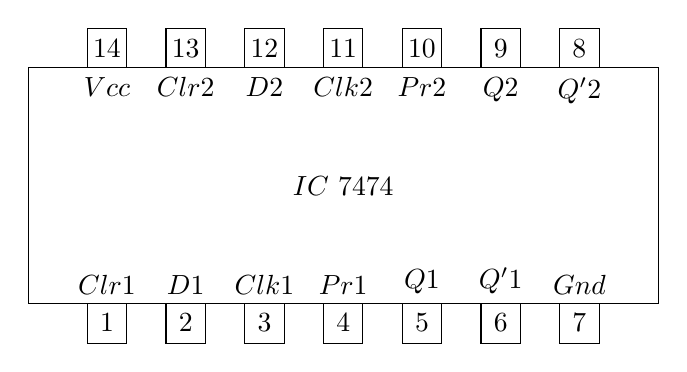
\begin{tikzpicture}
        \draw (0,2) rectangle (8,5);
        \draw (4,3.5) node{$IC$ $7474$};
        \draw (0.75,2) rectangle (1.25,1.5);
        \draw (1,2) node[below]{$1$};
        \draw (1,2) node[above]{$Clr1$};
        \draw (1.75,2) rectangle (2.25,1.5);
        \draw (2,2) node[below]{$2$};
        \draw (2,2) node[above]{$D1$};
        \draw (2.75,2) rectangle (3.25,1.5);     
        \draw (3,2) node[below]{$3$};
        \draw (3,2) node[above]{$Clk1$};
        \draw (3.75,2) rectangle (4.25,1.5);
        \draw (4,2) node[below]{$4$};
        \draw (4,2) node[above]{$Pr1$};
        \draw (4.75,2) rectangle (5.25,1.5);
        \draw (5,2) node[below]{$5$};
        \draw (5,2) node[above]{$Q1$};        
        \draw (5.75,2) rectangle (6.25,1.5);
        \draw (6,2) node[below]{$6$};
        \draw (6,2) node[above]{$Q'1$};
        \draw (6.75,2) rectangle (7.25,1.5);
        \draw (7,2) node[below]{$7$};
        \draw (7,2) node[above]{$Gnd$};
        \draw (0.75,5) rectangle (1.25,5.5);
        \draw (1,5) node[above]{$14$};
        \draw (1,5) node[below]{$Vcc$};
        \draw (1.75,5) rectangle (2.25,5.5);
        \draw (2,5) node[above]{$13$};
        \draw (2,5) node[below]{$Clr2$};
        \draw (2.75,5) rectangle (3.25,5.5);
        \draw (3,5) node[above]{$12$};
        \draw (3,5) node[below]{$D2$};
        \draw (3.75,5) rectangle (4.25,5.5);
        \draw (4,5) node[above]{$11$};
        \draw (4,5) node[below]{$Clk2$};
        \draw (4.75,5) rectangle (5.25,5.5);
        \draw (5,5) node[above]{$10$};
        \draw (5,5) node[below]{$Pr2$};
        \draw (5.75,5) rectangle (6.25,5.5);
        \draw (6,5) node[above]{$9$};
        \draw (6,5) node[below]{$Q2$};
        \draw (6.75,5) rectangle (7.25,5.5);
        \draw (7,5) node[above]{$8$};
        \draw (7,5) node[below]{$Q'2$};
    \end{tikzpicture}

		\caption{7474 Pin Diagram}
		\label{fig:2}
	\end{figure}

	The connections between Arduino UNO and two IC 7474 is given in below Table \\
	\begin{table}[h]
	\begin{center}
	\begin{tabular}{|c|c|c|c|c|c|c|c|c|}
        \hline & INPUT & \multicolumn{3}{|c|}{OUTPUT} & \multicolumn{2}{|c|}{CLOCK} & Vcc & GND \\
        \hline ARDUINO & D6 & D3 & D4 & D5 & \multicolumn{2}{|c|}{D2} & 5V & GND \\
        \hline 7447 && 5 & 9 && 3 & 11 & 14 & 7 \\
        \hline 7474 & 5 &&& 2 & \multicolumn{2}{|c|}{3} & 14 & 7 \\
        \hline
    \end{tabular}

	\end{center}
		\caption{Connections}
		\label{table:1}
	\end{table}

	The truth table for the circuit is given in below table \\
	\begin{table}[h]
		\begin{center}
	\begin{tabular}{|c|c|c|c|c|c|c|}
        \hline X & Y & Z & L1 & L2 & L3 & L3 \\
        \hline 0 & 0 & 0 & 1 & 1 & 1 & 1 \\
        \hline 0 & 0 & 1 & 1 & 1 & 1 & 1 \\
        \hline 0 & 1 & 0 & 1 & 1 & 1 & 1 \\
        \hline 0 & 1 & 1 & 1 & 0 & 1 & 1 \\
	\hline 1 & 0 & 0 & 1 & 1 & 1 & 1 \\
	\hline 1 & 0 & 1 & 1 & 1 & 1 & 1 \\
	\hline 1 & 1 & 0 & 1 & 0 & - & 1 \\
	\hline 1 & 1 & 1 & 1 & 1 & - & 1 \\
	\hline
        \end{tabular}

		\caption{Truth Table}
		\label{table:2}
		\end{center}
	\end{table}
	
	The Kmap for the circuit is \\
	\begin{figure}[h]
		\centering
	\begin{karnaugh-map}[4][2][1][$K$][$J$][$Qn$]
	\minterms{2,3,4,6}
	\autoterms[0]
	\implicant{3}{2}
	\implicantedge{4}{4}{6}{6}
\end{karnaugh-map}

	\caption{Kmap}
	\label{fig:3}
	\end{figure}

\section{Software}
	The Arduino code for the given circuit using IC 7474 is \\
	\lstinputlisting{gate2022.cpp}
\end{document}
